\section{FeatBench}
\subsection{Task Definition}

\begin{figure}[t]
    \centering
    \includegraphics[width=0.9\linewidth]{figs/benchmark.pdf}
    \caption{An overview of FeatBench. Each sample consists of four components.}
    \Description{A high-level architectural overview of a FeatBench task instance, illustrating the integration of four core components: 
    (1) Feature Description, which details the functional requirements;
    (2) Repository, representing the source code and repository structure; 
    (3) Execution Environment, depicting the containerized or isolated workspace for execution; 
    and (4) Evaluation Tests, showing the automated test suites used for verifying the implemented features against the design specifications.}
    \label{fig:benchmark}
\end{figure}

\begin{wrapfigure}{r}{0.45\linewidth}
    \vspace{-50pt}
    \centering
    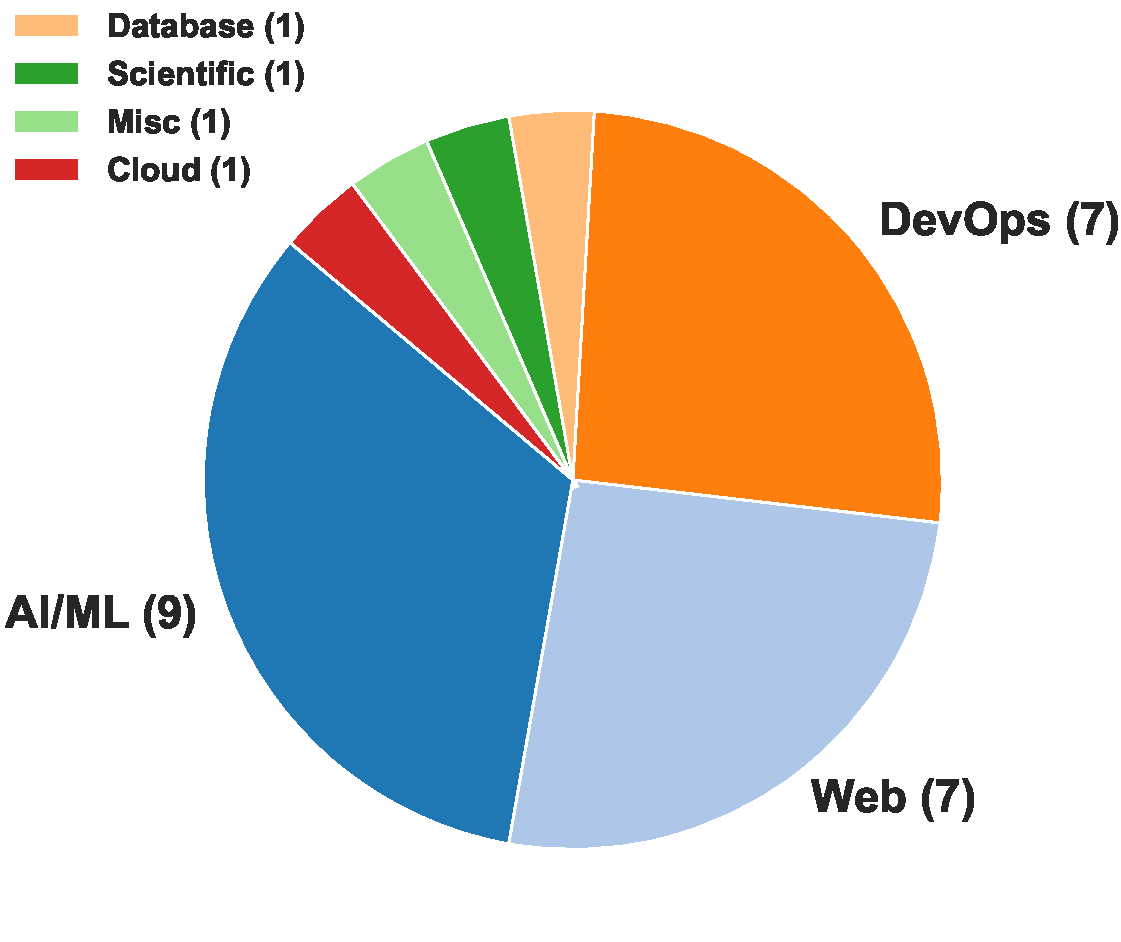
\includegraphics[width=\linewidth]{figs/category_pie.pdf}
    \caption{Repository distribution.}
    \Description{A pie chart illustrating the categorical distribution of the 27 open-source repositories included in FeatBench. The chart is divided into sectors representing different application domains, such as AI/ML, DevOps, Web development, and Database systems, showcasing the benchmark's diversity across various software ecosystems.}
    \label{fig:repo_distribution}
    \vspace{-20pt}
\end{wrapfigure}
\Cref{fig:benchmark} illustrates a sample task instance in FeatBench. Each instance comprises four key components: \ding{182} \textbf{Natural Language Requirements:} An abstract functional description strictly devoid of code hints, such as function signatures or file paths. This format mirrors realistic development scenarios, requiring agents to independently comprehend the repository context and devise a feature implementation strategy, thereby bridging the gap between high-level user intent and concrete code changes. \ding{183} \textbf{Running Environment:} A pre-configured Docker container providing a reproducible runtime environment with all necessary dependencies installed. \ding{184} \textbf{Repository:} The complete repository snapshot at the specific base commit, serving as the context for feature implementation. \ding{185} \textbf{Evaluation Tests:} A comprehensive test suite comprising F2P tests to verify the correctness of the new feature and P2P tests to ensure backward compatibility. Crucially, these ground-truth tests are withheld from the agent during inference to prevent data leakage.

\subsection{Features of FeatBench}

\paragraph{\textbf{Realistic Feature-level Code Generation without Hints.}} To mirror realistic software development scenarios, we formulate all task inputs as first-person feature requirements, typically initiating with phrases like ``I want to...''. Averaging 1,848 characters, these requirements are strictly devoid of code hints. Instead, they are structured to explicitly articulate the functional goals, background motivation, and specific requirements. This design ensures the agent receives a comprehensive context to guide autonomous development, while strictly isolating high-level user intent from code-level implementation consistent with real-world engineering practices.

\paragraph{\textbf{Evolving Data.}} To effectively mitigate data contamination, FeatBench is designed as an evolving benchmark. We develop and open-source a fully automated pipeline that constructs new benchmark versions from the latest repositories every six months. This automated process is highly cost-effective, with a processing cost of approximately \$0.28 per sample using DeepSeek V3.1. By continuously sourcing tasks from recent updates, we ensure that models are evaluated on novel, unseen data.

\paragraph{\textbf{Rigorous Data Collection Pipeline.}} We enforce strict quality assurance via a multi-level filtering pipeline that rigorously scrutinizes data at the repository, release, and Pull Request levels. At the repository level, we select actively maintained repositories. For the initial release of FeatBench, the cutoff date was set to June 2024. Candidate repositories are required to possess at least three formal releases and an identifiable test suite to guarantee verifiability. We also rigorously exclude repositories focused on tutorials or non-production code to ensure engineering relevance. At the Pull Request level, we impose stringent criteria to ensure testability, requiring that each task modifies at least one Python file and includes new or modified test cases. Crucially, we strictly restrict tasks to those modifying existing functions without adding or deleting functions. This constraint ensures that the developer-written test cases remain valid for evaluating generated code.

\paragraph{\textbf{Comprehensive Test Cases.}}
The correctness of each generated implementation is rigorously validated. On average, each task has 1694.6 test cases, comprising both F2P tests for feature verification and P2P tests for system stability. This extensive coverage not only validates the intended functionality but also robustly detects potential regressions, maintaining the reliability required for production-grade software.

\paragraph{\textbf{Diverse Application Domains.}}
Our benchmark encompasses a wide range of application domains, as detailed in \cref{fig:repo_distribution}. This diversity is designed to faithfully mirror the vast landscape of real-world software engineering, enabling a more realistic evaluation of agent capabilities within real-world development environments. We plan to continuously leverage our established pipeline to expand the benchmark, thereby broadening its alignment with a wider array of programming domains.

\subsection{Benchmark Construction Pipeline}

\begin{figure}[t]
    \centering
    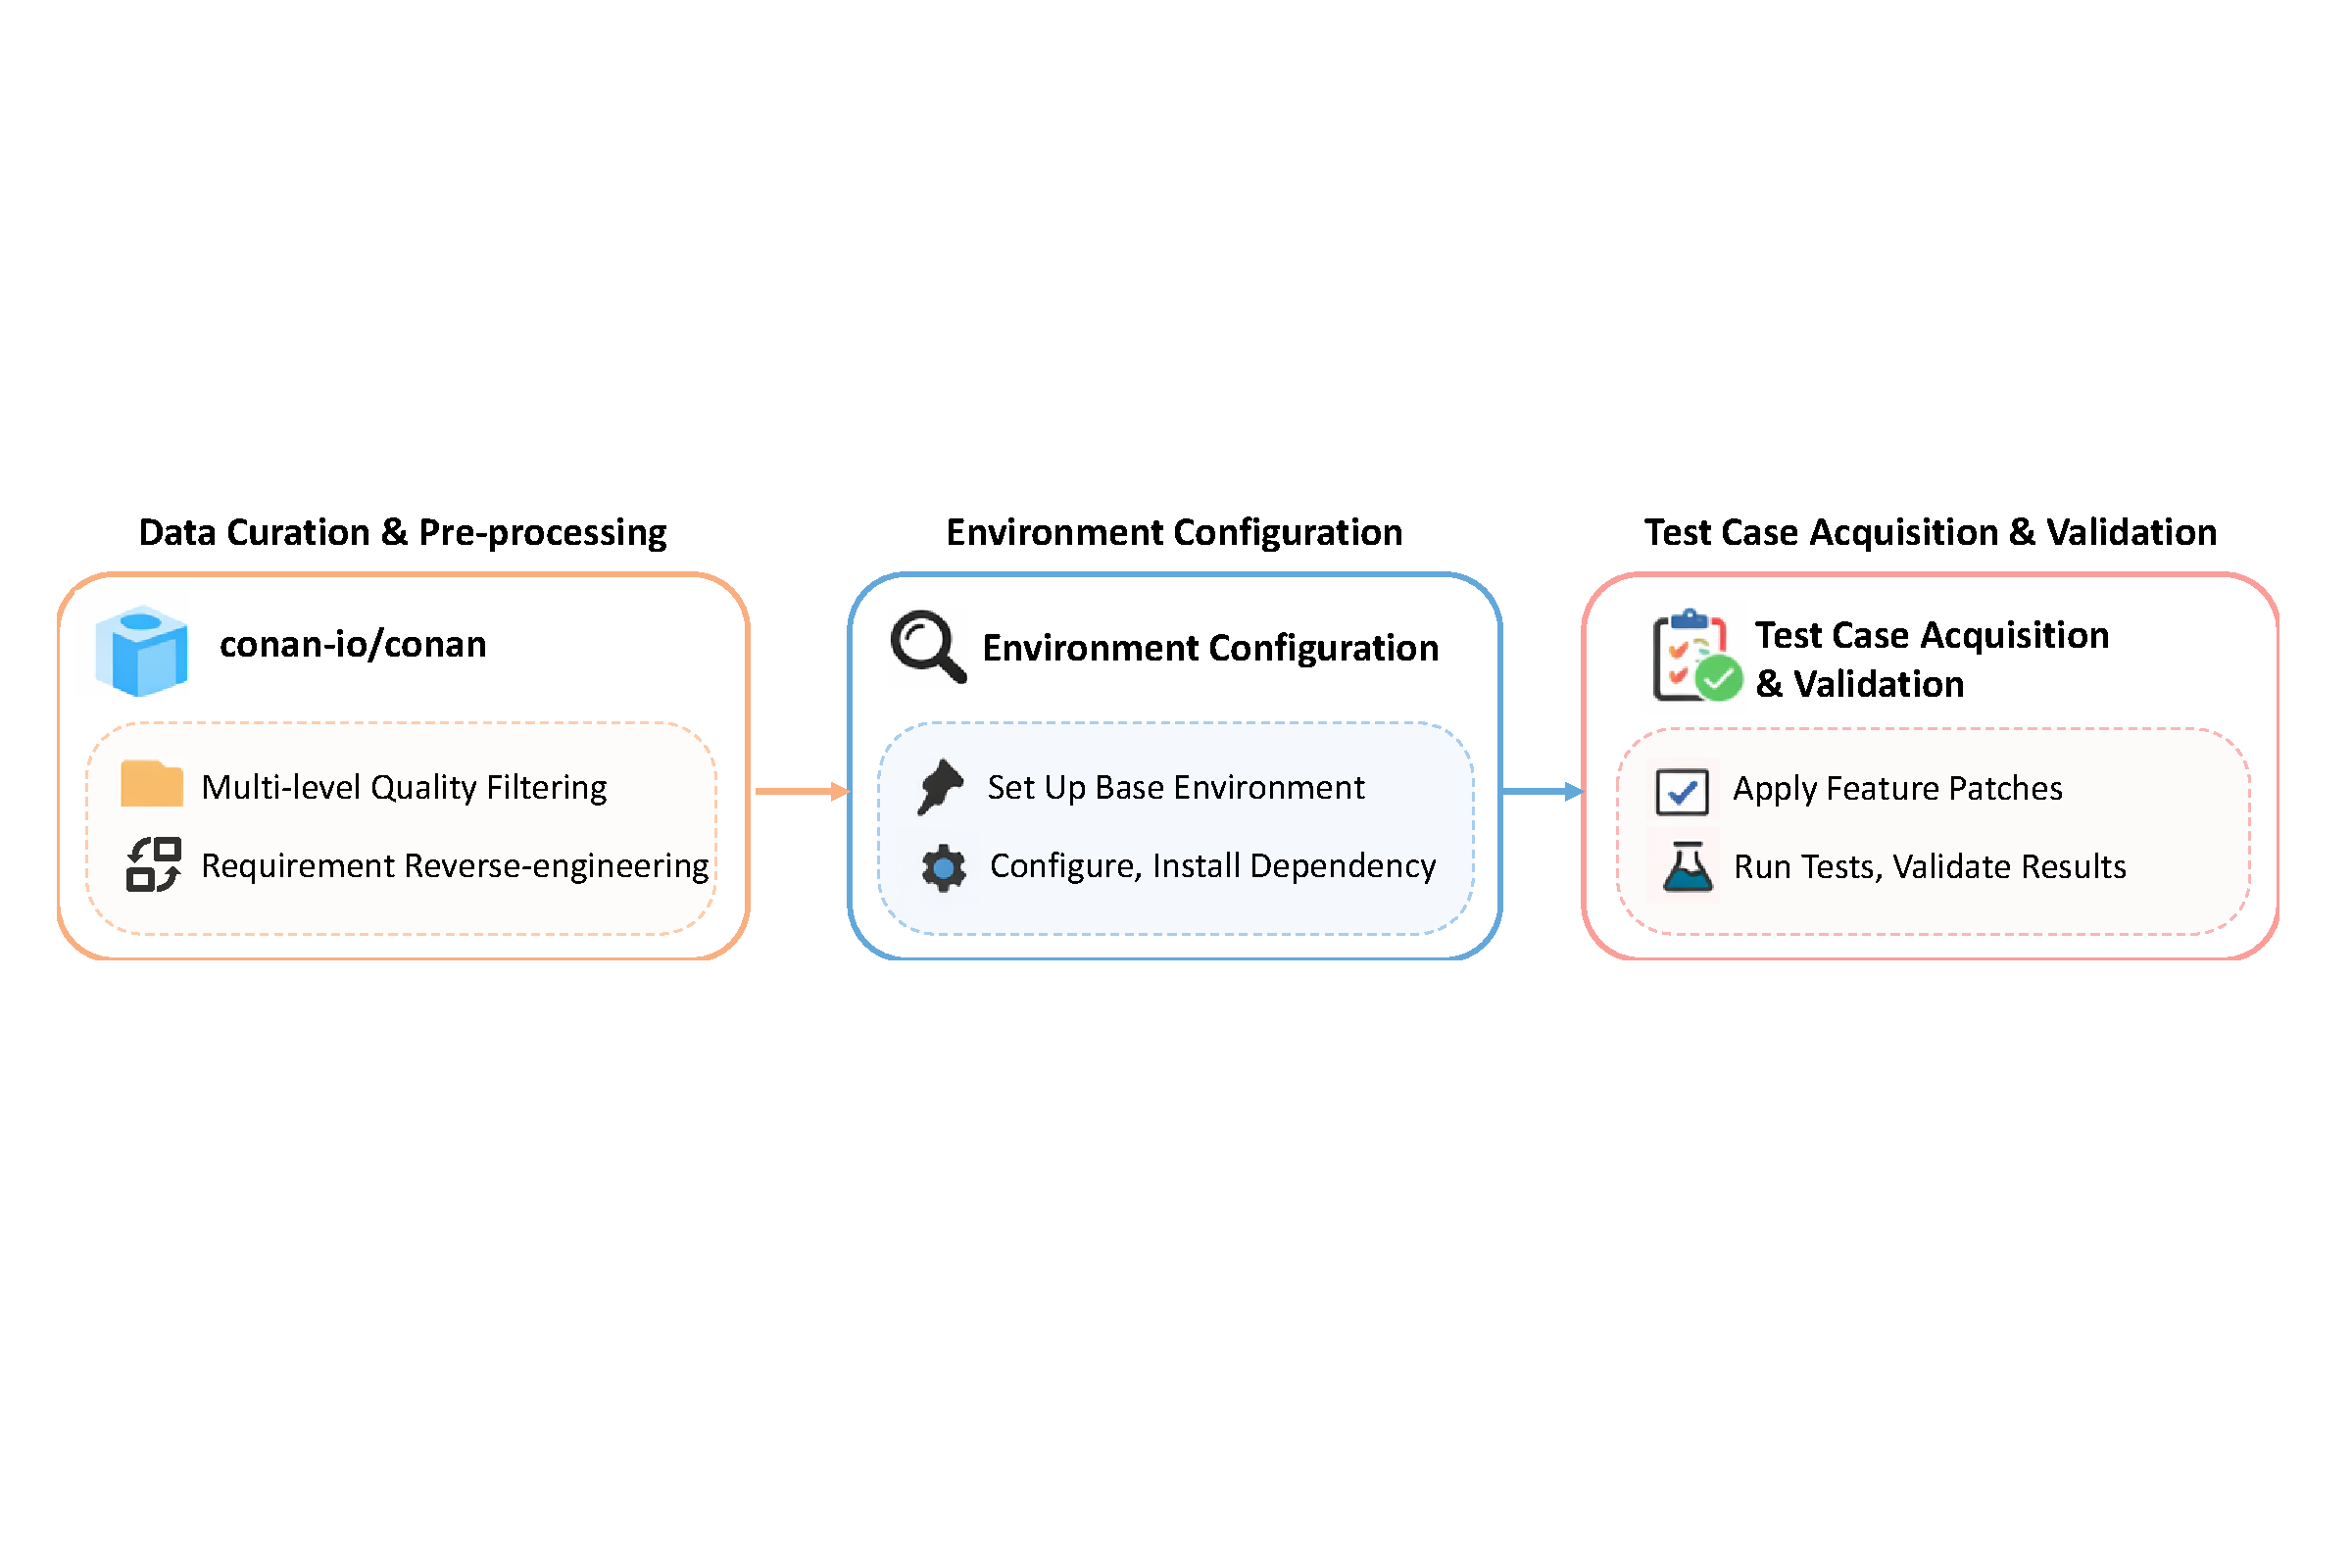
\includegraphics[width=\linewidth]{figs/pipeline_all.pdf}
    \caption{The pipeline of building our benchmark.}
    \Description{A flow diagram depicting the three-stage automated pipeline for constructing FeatBench.}
    \label{fig:pipeline}
\end{figure}

The FeatBench construction pipeline consists of three stages including data curation, environment configuration, and test case validation, as illustrated in \cref{fig:pipeline}. The pipeline initiates with data curation, utilizing multi-level filtering and reverse engineering to transform code changes into realistic requirements. This is followed by automated environment configuration, where an agent sets up base environment and installs dependency. The process concludes with test case acquisition and validation, extracting F2P and P2P tests from the repository to ensure functional correctness and backward compatibility.

\paragraph{\textbf{Stage 1: Data Curation and Pre-processing}}

\begin{wrapfigure}{r}{0.4\linewidth}
    \vspace{-10pt}
    \centering
    \includegraphics[width=\linewidth]{figs/pipeline_1.pdf}
    \caption{Data Curation and Pre-processing.}
    \Description{Data Curation, showing the filtering of repositories, releases, and Pull Requests.}
    \label{fig:pipeline_stage1}
\end{wrapfigure}

As illustrated in \cref{fig:pipeline_stage1}, the data curation and pre-processing stage includes a multi-level filtering and requirement reverse-engineering workflow. The initial filtering occurs at the repository level. To ensure data quality, the data curation process begins with a four-phase filtering criteria applied at the repository level: \ding{182} Repositories must have at least three formal releases to ensure a development history. \ding{183} They must possess an identifiable test suite (e.g., \texttt{tests/} directory) to enable automated validation. \ding{184} Content relevance is ensured by excluding repositories focused on tutorials, examples, or similar non-production code. \ding{185} For the initial release of FeatBench, we enforced a cutoff by considering only releases published after June 2024. Based on these strict standards, we selected 27 high-quality candidates from an initial pool of 44 open-source repositories.

Subsequently, we curated 675 releases from these repositories and analyzed them individually. First, we applied a filtering step to select releases created within the last year, longer than 30 characters, and that are not automated or trivial updates generated by bots. For these selected releases, we construct a comprehensive prompt that integrates the release title, description, and the repository's \texttt{README.md} file. We then instruct an LLM to categorize the contents of the release notes into \texttt{new\_features}, \texttt{improvements}, \texttt{bug\_fixes}, and \texttt{others}. While categorizing the content, we also ask the LLM to extract all relevant PR numbers from the text and associate them with the corresponding new feature entries. The prompt template is in \cref{sec:prompts}.

The final curation is applied at the PR level. From the filtered releases, we extracted an average of 3 feature-implementation PRs per release, yielding 297 high-quality samples. We retain only those meeting three specific criteria: \ding{182} The PR must modify at least one Python file. \ding{183} It must include new or modified test cases to ensure verifiability. \ding{184} The \textit{feature\_patch} must strictly modify existing functions without adding or deleting functions. This specific constraint on the \textit{feature\_patch} is crucial for testability, enabling static, developer-written test cases to validate the agent's implementation reliably. We posit this criterion is unbiased, reflecting scenarios where human developers refrain from altering function signatures due to maintenance concerns. The final validation step, ensuring each sample included at least one F2P test case, resulted in 157 tasks.

Finally, since real-world PR descriptions are often terse and developer-centric, we employ an LLM to reverse-engineer the original functional requirement from the code changes. The model is prompted to analyze the original PR title, description, and associated code changes (\textit{feature\_patch}) to generate a comprehensive and clear natural-language requirement. This augmented requirement simulates the realistic starting point of a feature implementation task without revealing technical details. To ensure the quality of these synthesized requirements, we conducted a human solvability assurance process in \cref{sec:human_eval}. This process verified their solvability and information completeness, effectively mitigating risks such as LLM hallucinations or the omission of critical implementation details. The reverse-engineering prompt template is in \cref{sec:prompts}. 

\begin{table}[t]
    \centering
    \caption{The required fields for our task instance. Fields marked with * are \textbf{newly added} in FeatBench compared to SWE-bench.}
    \resizebox{\textwidth}{!}{
    \begin{tabular}{c|c|p{10cm}}
        \toprule \texttt{Field}        & \texttt{Type}      & Description                                                                                                                                                                                                     \\
        \midrule \texttt{base\_commit} & \texttt{str}       & The commit on which the pull request is based, representing the repository state before the issue is resolved.                                                                                                  \\
        \texttt{patch}                 & \texttt{str}       & Gold patch proposed by the pull request, in \texttt{.diff} format.                                                                                                                                              \\
        \texttt{test\_patch}           & \texttt{str}       & Modifications to the test suite proposed by the pull request that are typically used to check whether the issue has been resolved.                                                                              \\
        \texttt{problem\_statement}    & \texttt{str}       & Issue description text, typically describing the bug or requested feature, used as the task problem statement.                                                                                                  \\
        \texttt{FAIL\_TO\_PASS}        & \texttt{List[str]} & Test cases that are expected to successfully transition from failing to passing are used to evaluate the correctness of the patch.                                                                              \\
        \texttt{PASS\_TO\_PASS}        & \texttt{List[str]} & Test cases that are already passing prior to applying the gold patch. A correct patch shouldn't introduce regression failures in these tests.                                                                   \\
        \texttt{*image\_key}           & \texttt{str}       & Instance-level docker image that provides an execution environment.                                                                                                                                             \\
        \bottomrule
    \end{tabular}}
    \label{tab:fields}
\end{table}

\paragraph{\textbf{Stage 2: Environment Configuration}}

\begin{wrapfigure}{r}{0.4\linewidth}
    \vspace{-10pt}
    \centering
    \includegraphics[width=\linewidth]{figs/pipeline_2.pdf}
    \vspace{-40pt}
    \caption{Environment Configuration.}
    \Description{Environment Configuration, illustrating the automatic generation of Docker images.}
    \label{fig:pipeline_stage2}
    \vspace{-10pt}
\end{wrapfigure}

As illustrated in \cref{fig:pipeline_stage2}, we develop an agent to configure the environment automatically. Inspired by SWE-bench-Live~\cite{swebenchgoeslive}, we construct a two-phase pipeline to configure the environment, mimicking the process of a human developer setting up an unfamiliar repository.

In the first phase, the analysis agent is tasked with information gathering. For each PR, it reverts the repository to its state before the PR (corresponding \textit{base\_commit}) and, guided by a pre-configured prompt, locates crucial files such as CI/CD configuration files (e.g., \texttt{.github/workflows}, \texttt{.travis.yml}), dependency definitions (e.g., \texttt{requirements.txt}, \texttt{pyproject.toml}), and \texttt{README.md} files. Simultaneously, it analyzes these configurations to determine the appropriate Python version for this PR. It ultimately outputs the detected version along with a structured file containing the paths to the top 20 most relevant environment configuration files for the subsequent configuration agent to use.

In the second phase, the configuration agent operates within a container launched from a base image corresponding to the identified Python version. This base image is pre-equipped with common development tools (e.g., \texttt{git}, \texttt{cmake}). To accelerate dependency installation and reduce build times, the agent uses both a caching mechanism and the high-performance package manager \texttt{uv} ~\cite{uv}. It is instructed to use the \texttt{--exclude-newer <commit\_timestamp>} parameter to enforce the use of package versions available at the time of the PR's creation. The prompt provided to the agent also includes troubleshooting heuristics, such as installing \texttt{pytest-timeout}~\cite{pytest-timeout} to prevent tests from hanging and ignoring specific internal test framework errors. Following this process, the agent systematically configures the environment, generating a test-ready image that accurately replicates the historical runtime environment. The agent's task is considered complete only after ensuring the PR's test suite is executable and installing all dependencies, including optional ones.

\paragraph{\textbf{Stage 3: Test Case Acquisition and Validation}}

\begin{wrapfigure}{r}{0.4\linewidth}
    \vspace{-10pt}
    \centering
    \includegraphics[width=\linewidth]{figs/pipeline_3.pdf}
    \caption{Test Case Acquisition and Validation.}
    \Description{Test Case Validation, demonstrating the extraction and verification of Fail-to-Pass and Pass-to-Pass test suites.}
    \label{fig:pipeline_stage3}
    \vspace{-10pt}
\end{wrapfigure}

This final stage establishes a robust ground truth for evaluation. F2P test cases are extracted from new or modified tests introduced in the current PR and serve as direct evidence of successful feature implementation. As illustrated in  \cref{fig:pipeline_stage3}, in a container initiated from the test-ready image, we first apply only the \textit{test\_patch}. We use Abstract Syntax Tree (AST) analysis on the \textit{test\_patch} to identify the specific tests added or modified for the new feature. We then selectively run these identified test cases by \texttt{pytest}~\cite{Pytest} and log the results, expecting them to fail. Next, we apply the \textit{feature\_patch} and rerun the same test cases, expecting them to pass. A PR is deemed valid, and the tests are confirmed as F2P only if any test case transitions from \texttt{FAILED/ERROR} to \texttt{PASSED}.

We also identify P2P test cases to prevent regressions. In the container, we first apply the \textit{test\_patch} and run all tests within the main test directory on the pre-patch repository, logging all passing cases. Subsequently, we apply the \textit{feature\_patch} and rerun all tests to confirm they still pass after the patch is applied. \Cref{tab:fields} summarizes the detailed definition of a constructed task instance.

\subsection{Dataset Statistics}
\begin{wraptable}{r}{0.38\textwidth}
    \vspace{-20pt}
    \centering
    \caption{Statistics of the repositories and task instances in FeatBench.}
    \label{tab:stats}
    \resizebox{\linewidth}{!}{
    \begin{tabular}{c|c|rr}
        \toprule
          \textbf{Level} & \textbf{\#Item} & \textbf{Average} & \textbf{Median} \\
          \midrule
          \multirow{3}{*}{\rotatebox[origin=c]{90}{Repo}}
            & Repositories & \multicolumn{2}{c}{27} \\
            & LoC & 209k & 106k \\
            & Files & 864 & 381 \\
          \midrule
          \multirow{6}{*}{\rotatebox[origin=c]{90}{Instance}}
            & Instances & \multicolumn{2}{c}{157} \\
            & Files\textsuperscript{*} & 2.4 & 2.0 \\
            & Hunks\textsuperscript{*} & 5.1 & 4.0 \\
            & Lines\textsuperscript{*} & 161.6 & 18.0 \\
            & F2P test cases & 2.2 & 1.0 \\
            & P2P test cases & 1692.4 & 1089.0 \\
        \bottomrule
        \multicolumn{4}{l}{\footnotesize{\textsuperscript{*}\textit{Stats of gold patch.}}}
    \end{tabular}}
    \vspace{-20pt}
\end{wraptable}

We present the detailed statistics of the constructed FeatBench in \cref{tab:stats}.
The benchmark comprises 157 task instances derived from 27 diverse, real-world open-source repositories.

As shown in the table, these repositories represent substantial engineering complexity, with an average size of 209k Lines of Code (LoC) and 864 files.
This scale requires agents to possess strong capabilities in repository-level context understanding and file localization.
Regarding the task granularity, the ground truth patches modify an average of 2.4 files and 5.1 code hunks per instance, reflecting the multi-file nature of authentic feature implementation.
Furthermore, to ensure rigorous evaluation, each instance is equipped with an extensive test suite.
On average, a task includes 2.2 F2P test cases to verify the new functionality and 1,692.4 P2P test cases to detect potential regressions robustly.